\chapter{Contexte général du projet}


\section{Organisme d’accueil}


Le Groupe BCP est un groupe financier panaricain et universel au service de toutes les catégories socio-professionnelles. À vocation inclusive, il offre à ses clients particuliers, professionnels et entreprises de toutes tailles, des produits bancaires, d’assurance et de service. \\
La Banque Centrale Populaire constitue l’organe central du Groupe, qui se compose de huit Banques Populaires Régionales (BPR), de trois fondations et de plusieurs filiales au Maroc et à l’international.

\begin{figure}[H]
    \centering
    
\includegraphics[width=.75\textwidth]{logos/BCP.png}
    \caption{Logo de la Banque Populaire}
\end{figure}

\subsection{Aperçu historique}
Fondée en 1961, la BCP a rapidement émergé comme leader du marché des dépôts au Maroc, atteignant 1 milliard de dirhams en 1974. En 1980, elle comptait déjà  \\ 500 000 clients et 5 milliards de dirhams en dépôts. La BCP a réalisé son ambition d’expansion à l’international en créant la Banque Chaabi du Maroc à Paris et une succursale à Bruxelles en 1976. En 2000, elle s'est transformée en société anonyme à conseil d'administration et a été cotée à la Bourse de Casablanca en 2004.
\\ \\
Le développement de la BCP s'est poursuivi avec des investissements stratégiques et une expansion continue. En 2015, la banque a porté ses participations dans les BPRs à 52 \%, devenant ainsi majoritaire. Dans la même année, la BCP a enregistré une augmentation de 14,4 \% de son résultat net, atteignant 2,5 milliards de dirhams et 5,2 millions de clients.  \\  
En 2020, la Banque Populaire a participé  avec une contribution d'un milliard de dirhams au fonds de lutte contre le coronavirus fondé par le Roi Mohammed VI. 


\subsection{Structure organisationnelle}
La Banque Centrale Populaire se distingue par une structure organisationnelle solide et stratégiquement pensée, reflétant son engagement envers l'excellence opérationnelle, la gouvernance efficace et la satisfaction des clients. 
\\ \\
Cette organisation, fruit d’un travail de co-construction avec les instances de gouvernance du Groupe et l’équipe dirigeante, s’articule autour de:
\\

\begin{itemize}
    \item  \textbf{Direction Générale Banque Commerciale}: structurée autour d’entités Producteurs par segment de clientèle (Particuliers, Professionnels, Marocains Du Monde, TPE, PME et GE) et d’entités Distributeurs, au Maroc et dans les pays de
    présence en Europe, au Moyen Orient et en Amérique;
    \\
    \item \textbf{Direction Générale BCP et International}: structurée autour, d’une part, d’entités Plateformes Produits et Services, spécialisées
    et mutualisées à l’échelle du Groupe et, d’autre part, de la Banque de l’International en charge du développement et du pilotage des activités du Groupe en Afrique Subsaharienne, au Moyen Orient et dans l’Océan Indien.
    \\
    \item  \textbf{Direction Générale Risques Groupe}: structurée
    autour des filières de maîtrise et de gestion des risques ayant une portée Groupe,
    menant une triple mission: normative, de contrôle et de service;
    \\
    \item Consolidation du positionnement stratégique, en rattachement à la \textbf{Présidence Direction Générale}, des fonctions en charge des \textbf{Finances et Performances Groupe}, de la \textbf{Stratégie Groupe}, de la \textbf{Conformité et du Développement Durable}, ainsi que celles inhérentes à la \textbf{Marque, Capital Humain \&Gouvernance Groupe}.
\end{itemize}

\begin{figure}[H]
    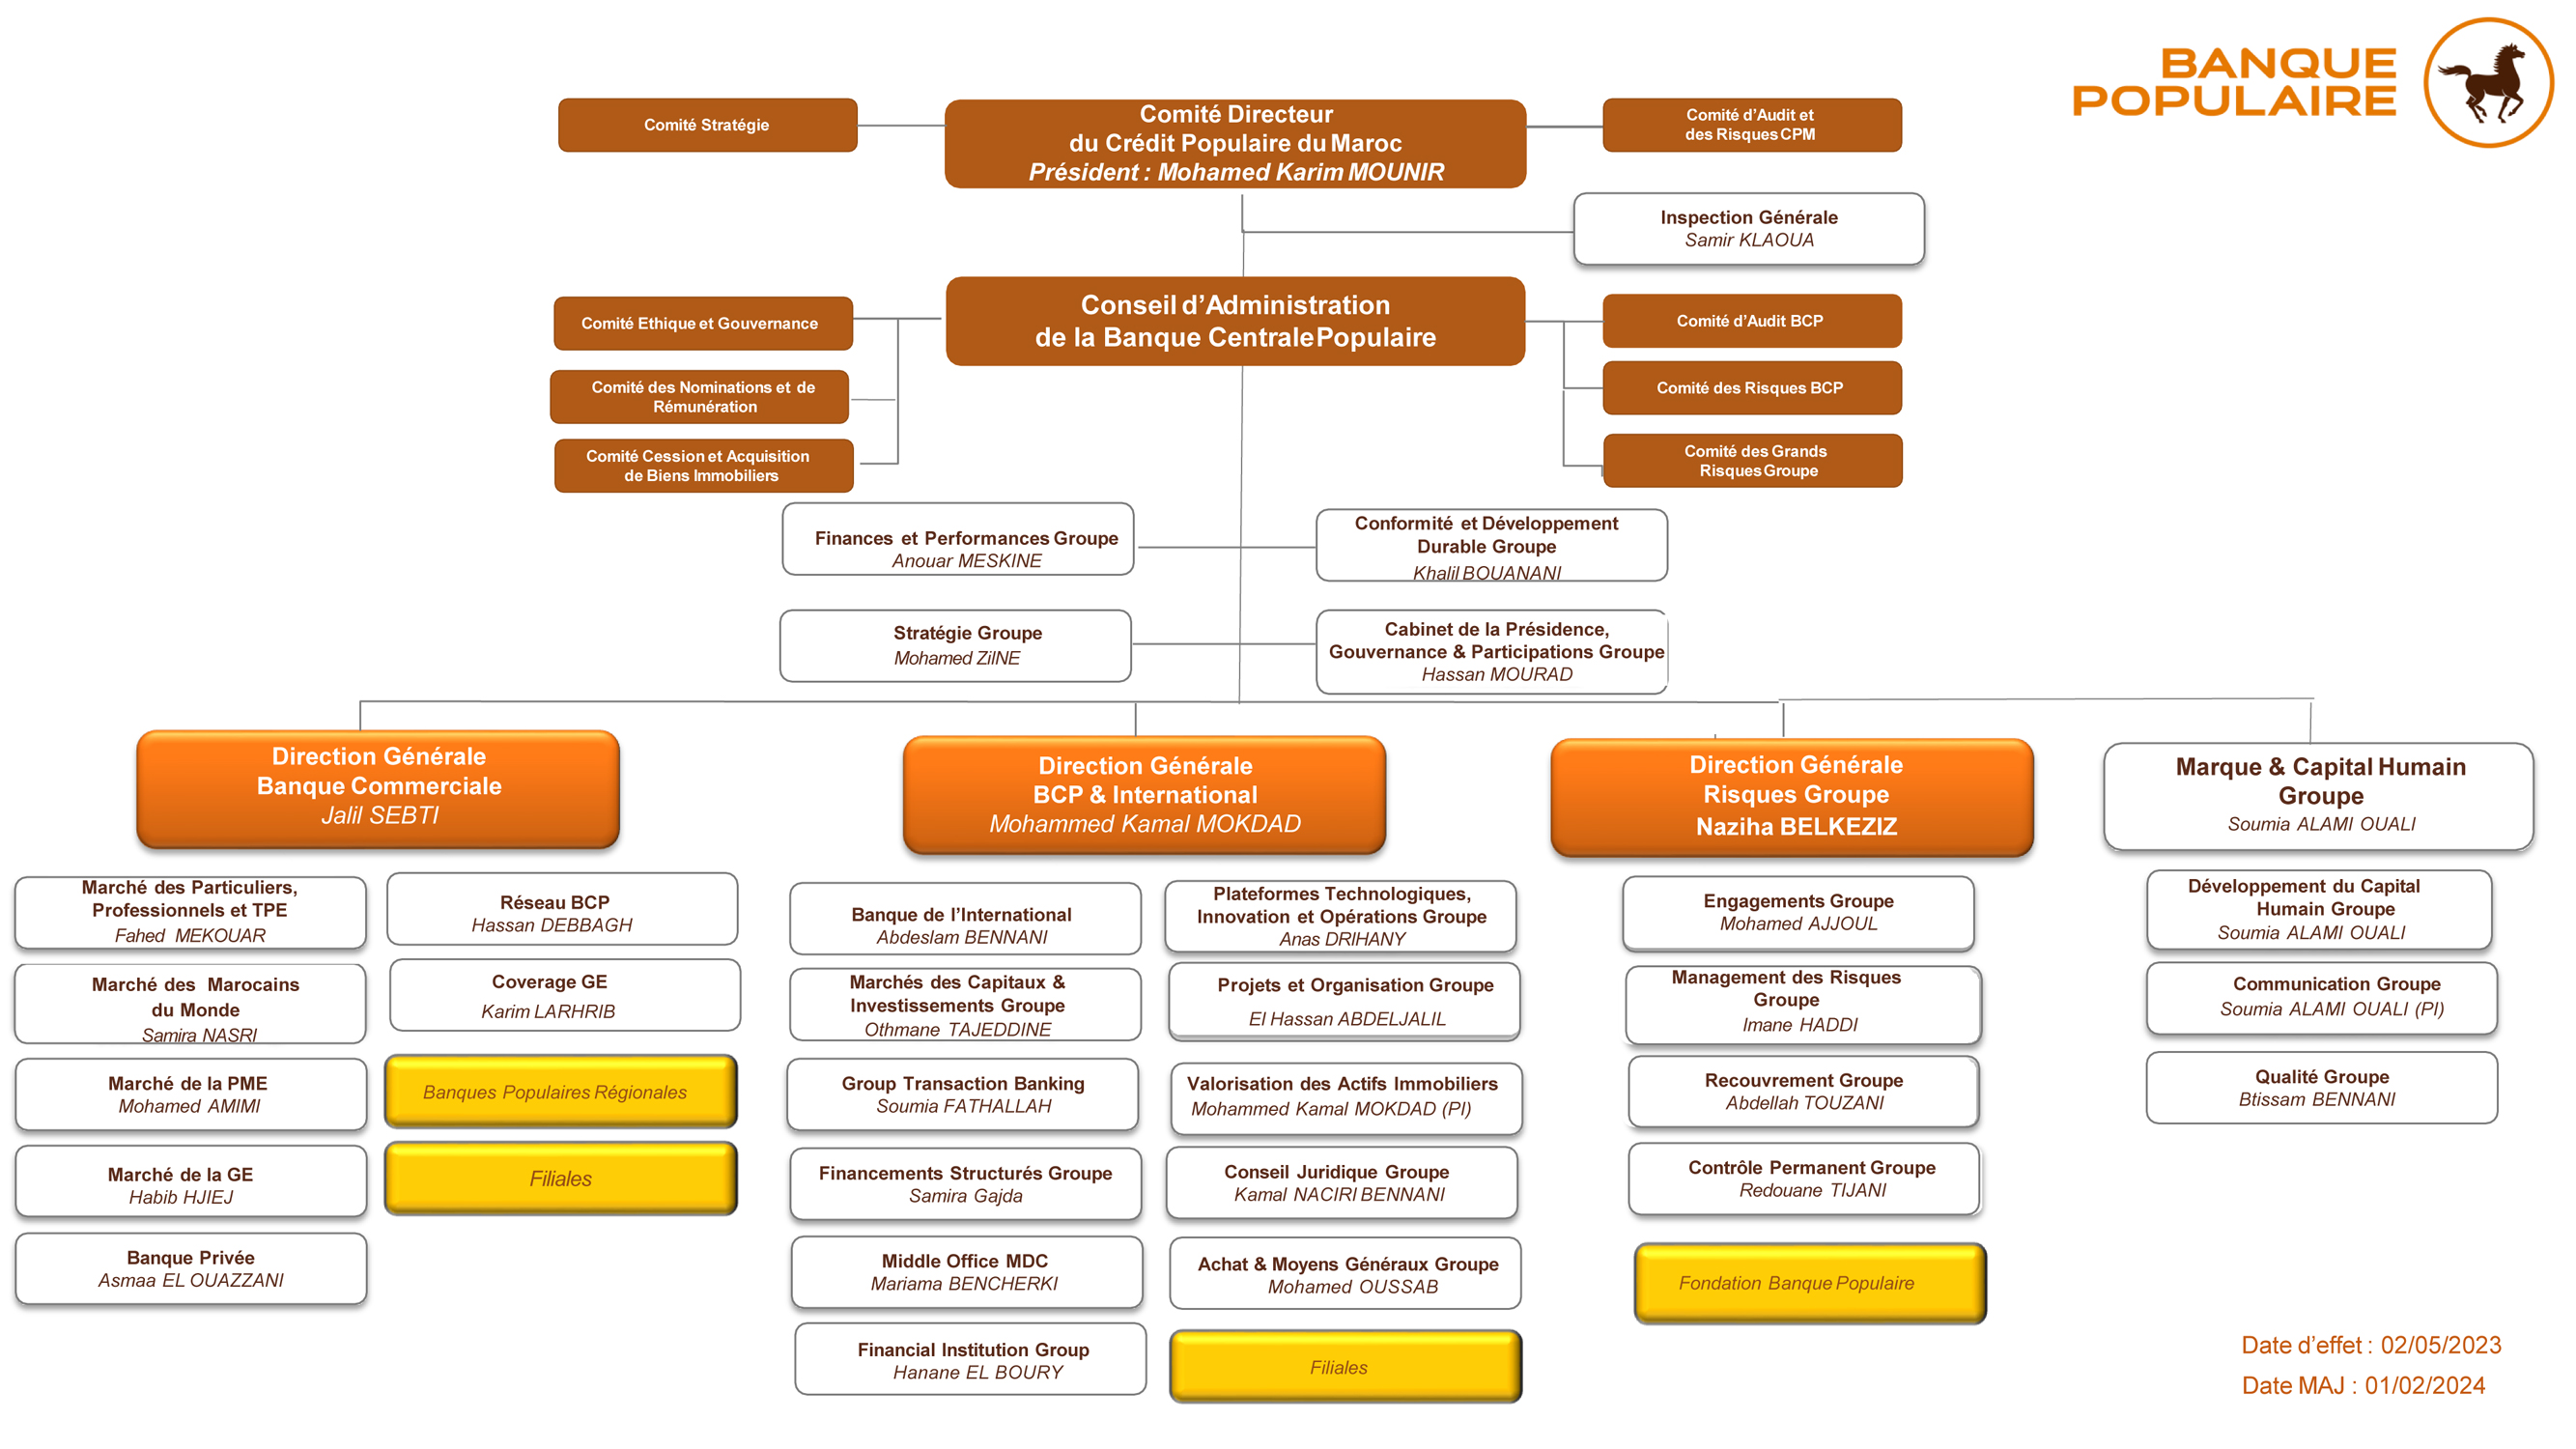
\includegraphics[height=.52\textheight, angle=90, origin=c]{images/bcp-structure.jpg}
    \caption{Organigramme du groupe BCP}
\end{figure}

\clearpage

\subsection{Missions et valeurs}

\subsubsection{Missions}
Les missions de la Banque Centrale Populaire peuvent être divisées en deux piliers principaux:

\begin{itemize}
    \item Réaliser toutes les opérations bancaires pour lesquelles elle est habilitée en tant qu'établissement de crédit et coordonner la politique financière du Groupe.
    \item Incarner l'organisme central bancaire des Banques Populaires Régionales en assurant leur refinancement, la gestion de leurs excédents de trésorerie et les services d'intérêt commun pour ses organismes.
\end{itemize}

\subsubsection{Valeurs}
Les valeurs de la BCP sont au cœur de son identité et de ses actions. Elles guident ses décisions, inspirent ses équipes, et assurent une relation de confiance avec ses clients et partenaires. Celles-ci incluent:

\begin{itemize}
    \item \textbf{Proximité}: Valeur historique de la Banque Populaire, reflète son héritage coopératif et son ancrage local. Elle consiste à écouter et comprendre les besoins des clients, collaborateurs et partenaires pour adapter ses offres et sa stratégie d'expansion locale. Cette approche garantit la pertinence et la réactivité de ses actions sur le terrain;
    \item \textbf{Citoyenneté}: Se manifeste par un engagement responsable envers les communautés, les partenaires et les écosystèmes où la Banque Centrale Populaire opère. Elle se traduit par la promotion de l'intérêt collectif dans toutes ses initiatives et ses choix;
    \item \textbf{Performance}: Stratégiee définit par la création de valeur durable pour les clients, collaborateurs, actionnaires et partenaires. Cela se matérialise par un engagement collectif pour atteindre notre ambition commune;
    \item \textbf{Innovation}: Se caractérise par une réinvention continue de la proposition de valeur, des modes de fonctionnement et de communication, tout en cultivant l'humilité. Elle implique la création d'un environnement de confiance favorable à l'expression de la créativité et à l'audace.
\end{itemize}


\clearpage



\section{Présentation du projet}

\subsection{Client: Fonction Conformité Groupe}
En référence aux meilleures pratiques et aux recommandations de la directive de Bank Al-Maghrib n°49/G, le Groupe s'est doté, au début de l'exercice 2007, d'une fonction "Conformité". Celle-ci a pour mission principale le contrôle permanent de dernier ressort de l'application des lois, réglementation et normes en vigueur, afin de renforcer son système de gouvernance et la confiance des marchés ainsi que d'asseoir son processus de développement aussi bien sur le marché national qu'à l'international.\\

\noindent Le périmètre d'action de cette fonction couvre quatre activités principales : la conformité réglementaire, la déontologie et la gouvernance, la lutte anti-blanchiment et due diligence ainsi que la supervision du système de contrôle interne du Groupe.\\

\noindent A ce titre, et à fin de respecter les exigences de la CNDP en matière de traitements des données à caractère personnel, la fonction conformité a exprimé le besoin d'automatisation du registre du traitement.

\subsection{Problèmatique}
Conformément aux directions de la CNDP, la BCP est tenue de maintenir un registre qui décrit l'ensemble des traitements des données à caractère personnel effectuées par la banque. Chaque traitement doit faire l'objet d'une fiche qui permet d'identifier le traitement et la nature des données sur lesquelles il opère. \\ 

\noindent Actuellement, la tenue du registre de traitement est réalisée à l'aide de fichiers Excels dont la manipulation, la validation, et la consultation comprend un nombre de taches répététives qui présentent un risque augmenté d'erreur, de mal-pratique, et un coût élevé en matière de temps et de ressources.\\

\noindent Face à ces contraintes, le besoin d'automatisation du registre de traitement s'avère non-seulement pertinent mais également impératif.

\subsection{Objectif}
Le projet vise à développer une application web qui permettra d'automatiser les processus liées à la gestion du registre du traitement, et ce afin d'assurer la conformité réglementaire de la BCP vis-à-vis les directions de la CNDP concernant les traitements des données à caractère personnel. 

